The ultimate challenge of any deployment life cycle is tying all ideas into a single, nicely wrapped package. This is the goal of orchestration.
To implement, or \textit{orchestrate} a deployment such as this, we designed a multi-tiered architectural diagram (Figure~\ref{fig:architecture})
that outlines how every building block in our environment fits together to form a finalized representation of a working project. 

% Add the figure
\begin{figure}[h]
    \centering
    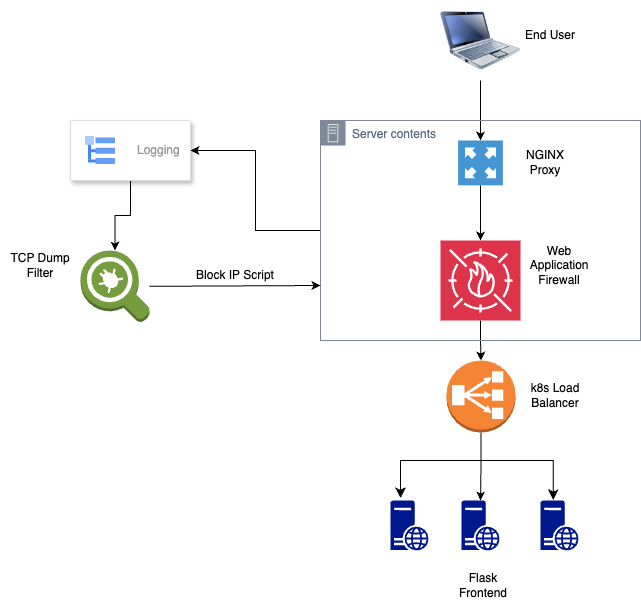
\includegraphics[width=\columnwidth]{resources/diagram.png} 
    \caption{Multi-tiered architectural diagram.}
    \label{fig:architecture}
\end{figure}

To host our content, we utilized Kubernetes. This method first involved integrating a docker image that was specifically designed to host content created by our frontend developers.
We then created service and deployment YAML files to control multiple containers behind a load balancer. 

Once we had a functional cluster of orchestrated containers, the next goal was to make our load balancer not the first point of contact between external users and our internal environment. 
This involved integrating an NGINX reverse proxy ~\cite{nginx} on our host machine to facilitate communication without exposing our services directly to the internet. 

To setup an NGINX reverse proxy, we had to install the service then modify the global configuration file in the \texttt{/etc/nginx/conf.d/} directory to specifically mediate communications between external users and our internal load balancer ~\cite{hostinger_nginx_proxy}. The specifics for this step is
very convoluted, essentially we had to define server and location blocks with a \texttt{proxy pass} flag to enable the proxy feature of NGINX.

To tie our scalable, secure environment together on the orchestration end, we installed a web application firewall (WAF) on our reverse proxy to inspect requests being sent to the load balancer ~\cite{linode_modsecurity}. The requests
will be meticulously cross-referenced against a series of rule lists specifically designed to catch exploits matching the OWASP Top Ten vulnerabilities. If a exploit request is detected, the WAF will drop the request and return
a HTTP 403 status code to the threat actor.
